\subsection{Database e modelli}
Il database utilizzato per lo sviluppo del progetto è stato \textbf{Sqlite}, scelto per la
sua leggerezza e facilità di utilizzo. Nulla impedisce però di potersi spostare ad
altri database in caso di nuovi futuri requisiti.
\\I modelli (tabelle) utilizzati all’interno del database sono stati:

\subsubsection{User}
Modello usato per gestire le tipologie di utenti che possono utilizzare il sito. Per
la realizzazione è stato esteso il modello AbstractUser, presente nell’insieme di
classi messe a disposizione dal framework Django, in modo da avere già diversi
campi disponibili per l’uso.

\begin{center}
  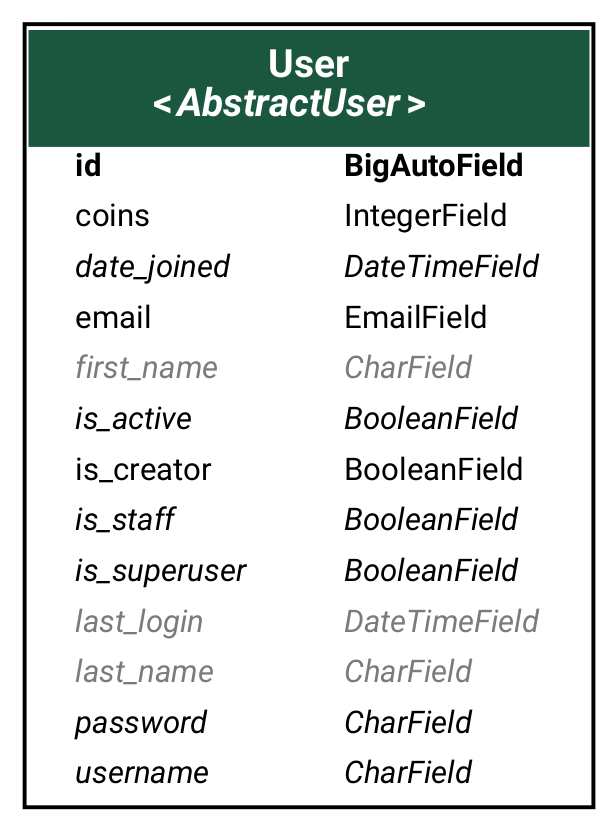
\includegraphics[width=0.4\linewidth]{images/user.png}
\end{center}

\subsubsection{CoinsPurchase}
Modello usato per registrare le transazioni di acquisto di monete di un utente.
Ha utente come chiave esterna per identificare l’utente che ha effettuato la transazione.
\begin{center}
  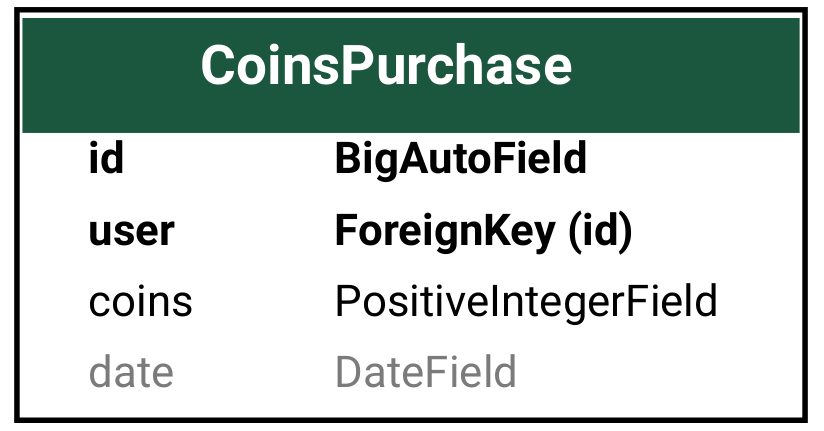
\includegraphics[width=0.4\linewidth]{images/coins-purchase.png}
\end{center}


\subsubsection{Genre}
Modello usato per gestire i generi dei comics.
\\È stato scelto di utilizzate una tabella a se stante in vista di eventuali inserimenti di nuovi generi.

\begin{center}
  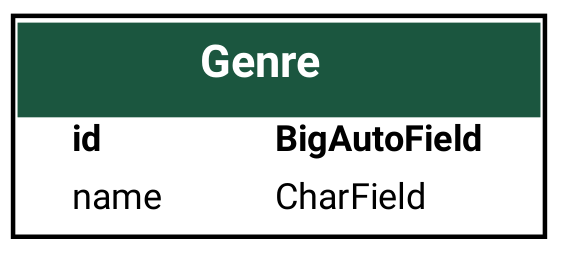
\includegraphics[width=0.4\linewidth]{images/genre.png}
\end{center}


\subsubsection{Comic}
Modello usato per gestire i dati di uno specifico comic.
Ha utente come chiave esterna per identificare l’utente che ha caricato il comic.
I campi follows, rating e watches vengono aggiornati in automatico.
Le immgini delle cover vengono salvate in una cartella che viene creata in
caso non esista.
\\La tabella \textbf{Comic} ha una relazione Many-to-Many con la tabella \textbf{Genre}, siccome un comic può avere più generi.

\begin{center}
  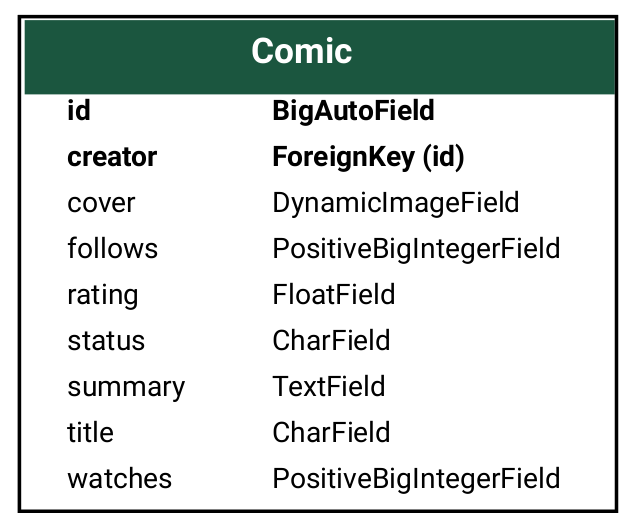
\includegraphics[width=0.4\linewidth]{images/comic.png}
\end{center}

\subsubsection{Chapter}
Modello usato per gestire i dati di un capitolo di uno specifico comic.
Anche in questo caso il campo like viene aggiornato in automatico.
\\La colonna \textbf{chapter-num} indica il numero del capitolo relativamente al comic.


\begin{center}
  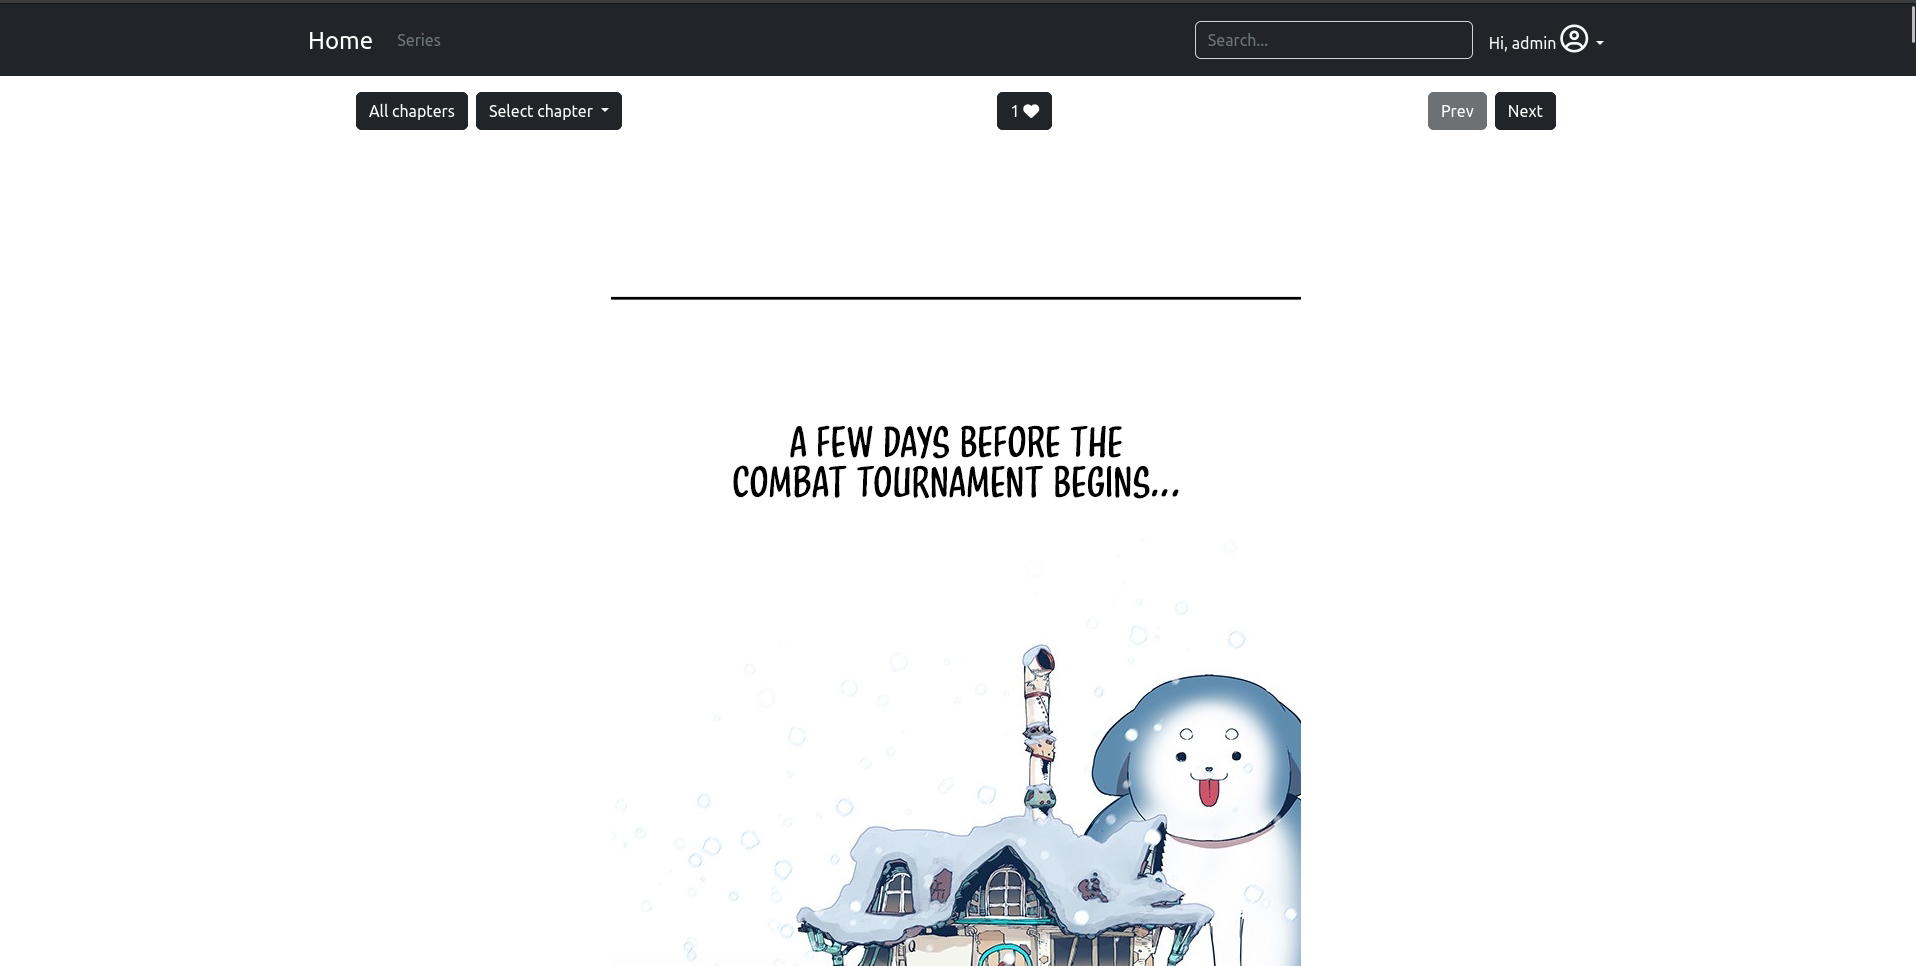
\includegraphics[width=0.4\linewidth]{images/chapter.png}
\end{center}

\subsubsection{ChapterImage}
Modello usato per gestire le immagini di un capitolo di uno specifico comic.
È stato utilizzato un modello a se stante siccomene il numero di immagini inseribili non è stato limitato.

\begin{center}
  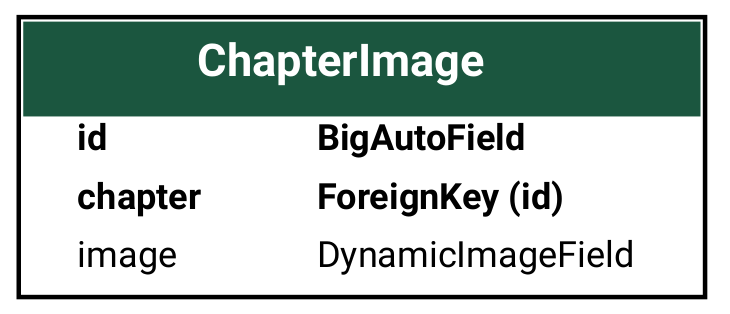
\includegraphics[width=0.4\linewidth]{images/chapter-image.png}
\end{center}

\subsubsection{BuyList}
Modello usato per gestire i capitoli acquistati da ogni utente.
Il modello è utile per consentire l'accesso ad un capitolo ai soli utenti che lo hanno acquistato.

\begin{center}
  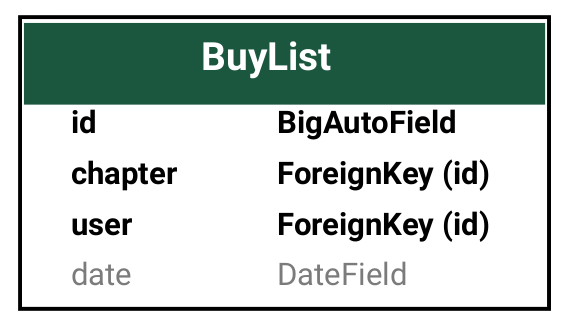
\includegraphics[width=0.4\linewidth]{images/buy-list.png}
\end{center}

\subsubsection{Rating}
Modello usato per gestire i voti di un utente ad un deteminato comic.
L'utilità del modello sta nel fatto che permette la modifica e la rimozione del voto da parte di un utente.

\begin{center}
  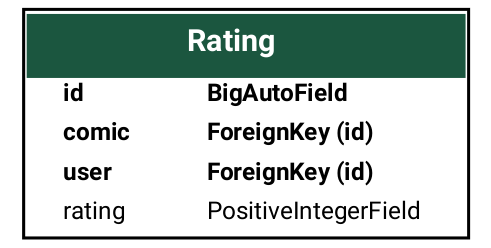
\includegraphics[width=0.4\linewidth]{images/rating.png}
\end{center}

\subsubsection{Like}
Modello usato per gestire i like di un utente ad un deteminato capitolo.
Come per il Rating, questo modello permette l'aggiunta e la rimozione di likes.

\begin{center}
  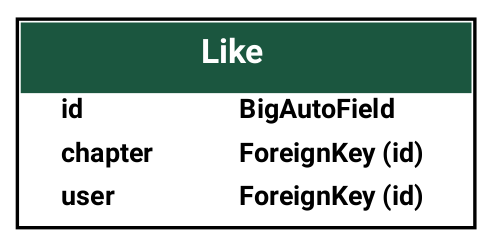
\includegraphics[width=0.4\linewidth]{images/like.png}
\end{center}

\subsubsection{Library}
Modello usato per gestire la libreria di comic di un utente.

\begin{center}
  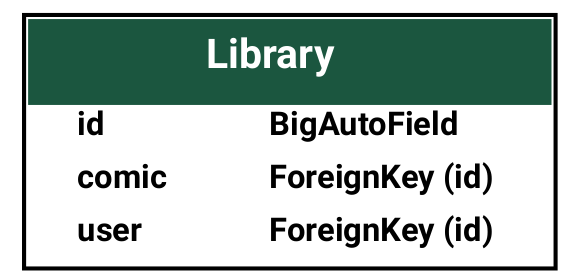
\includegraphics[width=0.4\linewidth]{images/library.png}
\end{center}

\subsubsection{ReadHistory}
Modello usato per gestire la cronologia di lettura di un utente.

\begin{center}
  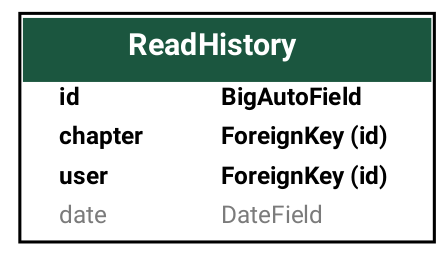
\includegraphics[width=0.4\linewidth]{images/history.png}
\end{center}

\subsubsection{Comment}
Modello usato per gestire i commenti di un utente ad un determinato capitolo.
Questo modello ha il campo \textbf{reply-to} che permette di rispondere ad altri commenti.

\begin{center}
  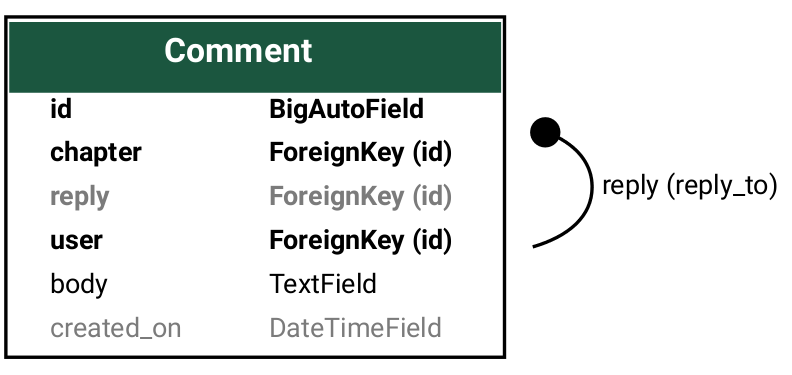
\includegraphics[width=0.4\linewidth]{images/comment.png}
\end{center}


\subsubsection{Modelli app comics}
\begin{center}
  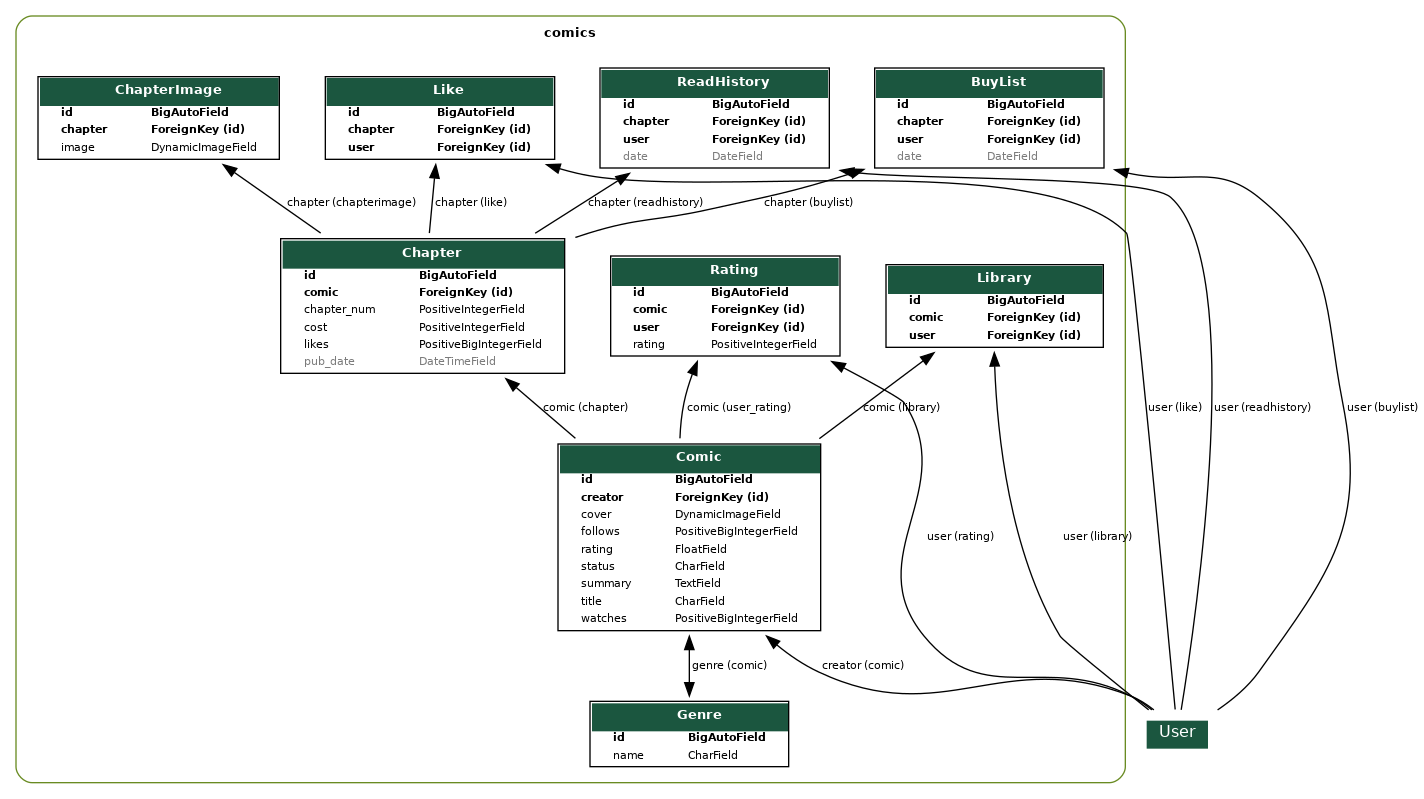
\includegraphics[width=1.0\linewidth]{images/comics.png}
\end{center}

\subsubsection{Modelli app users}
\begin{center}
  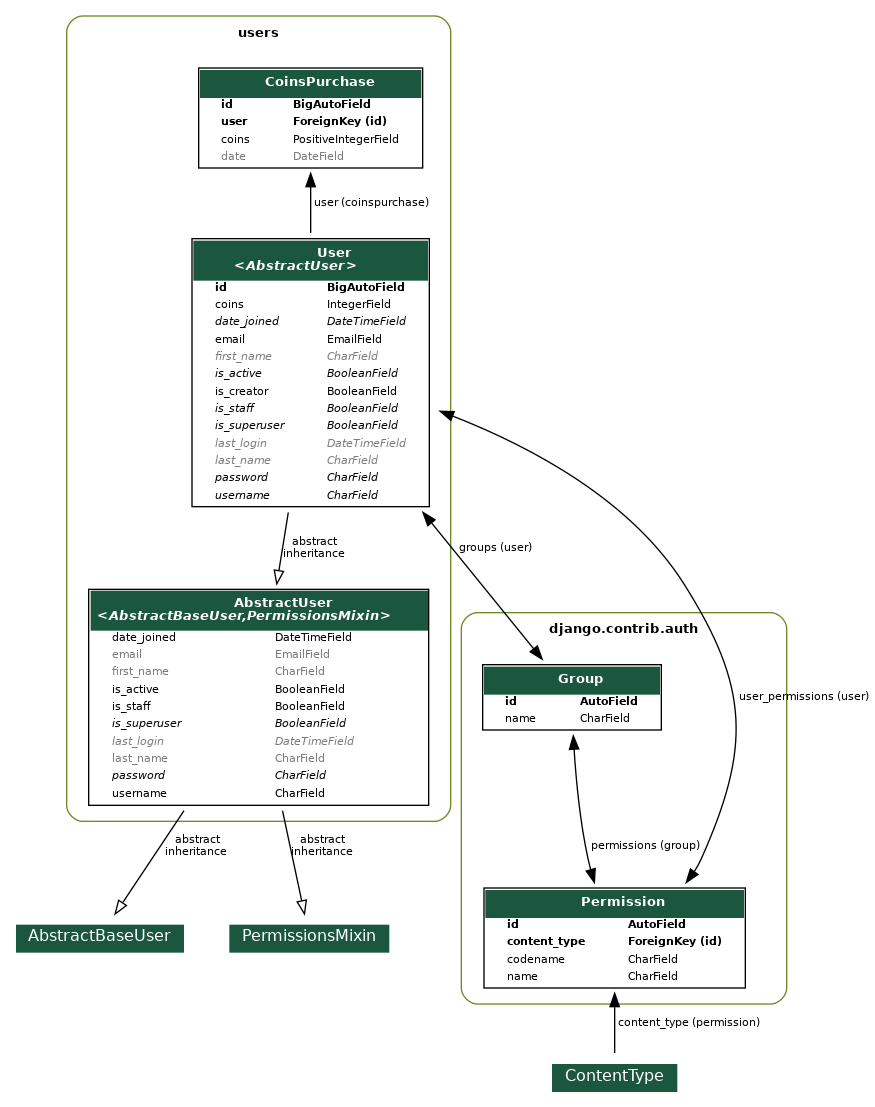
\includegraphics[width=1.0\linewidth]{images/users.png}
\end{center}

\subsubsection{Modelli app comment}
\begin{center}
  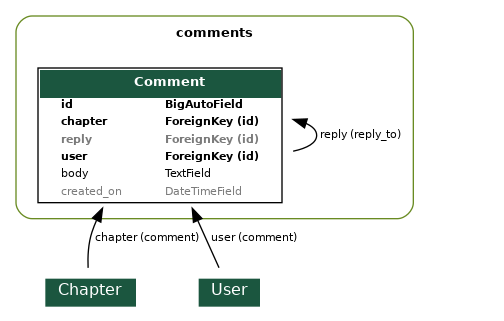
\includegraphics[width=1.0\linewidth]{images/comments.png}
\end{center}

\subsubsection{Schema completo}
\begin{center}
  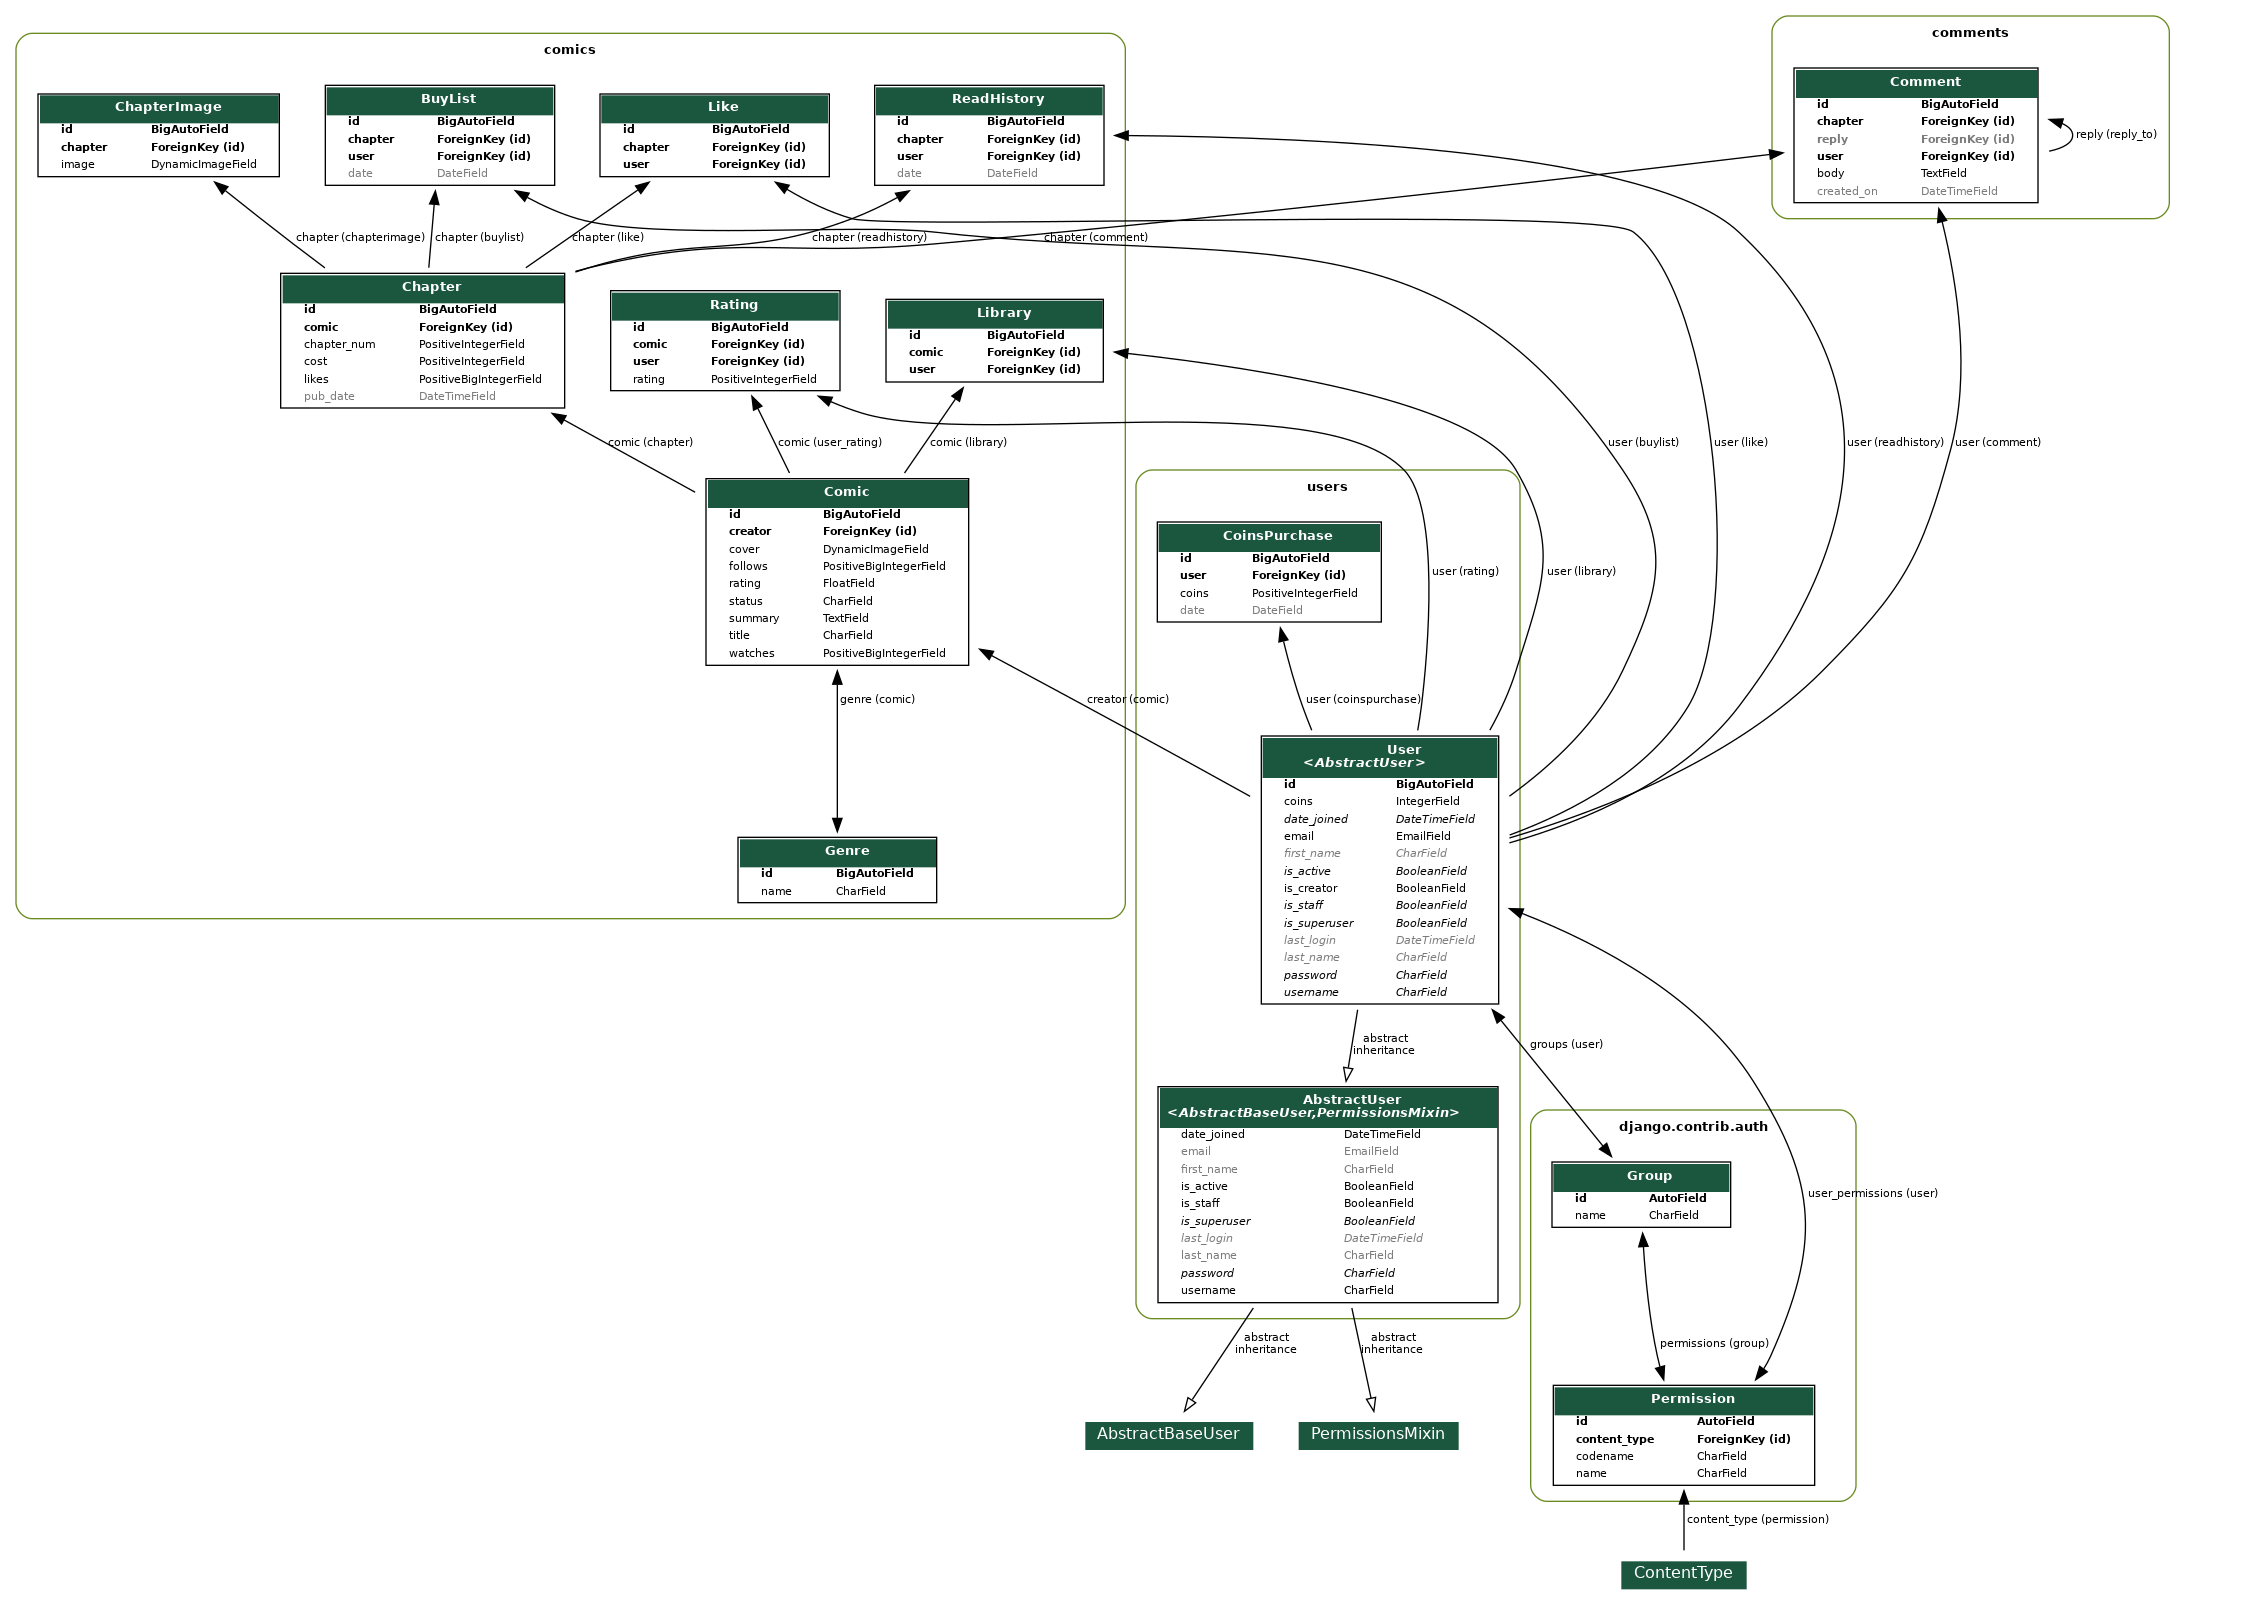
\includegraphics[width=1.3\linewidth, angle=90]{images/project.png}
\end{center}